\documentclass[krantz1]{krantz} %See documentation for other class options
\usepackage{fixltx2e,fix-cm}
\usepackage{amssymb}
\usepackage{amsmath}
\usepackage{graphicx}
\usepackage{subfigure}
\usepackage{makeidx}
\usepackage{multicol}

%\usepackage[dvips]{hyperref}


\makeindex

\newtheorem{theorem}{Theorem}[chapter]
\newtheorem{exercise}{Exercise}[chapter]
\newtheorem{example}{Example}[chapter]
\newtheorem{definition}{Definition}[chapter]
%%\newtheorem{proof}{Proof}
\newenvironment{proof}[1][Proof]%
%  \topsep6\p@\@plus6\p@ \trivlist
{\par\addvspace{6pt}\normalfont {\bfseries #1}\hskip\labelsep\ignorespaces\itshape}
{\par\addvspace{6pt}}
 %place custom commands and macros here

\begin{document}

\frontmatter

\title{Krantz Template} %This is a placeholder titlepage, it will not be final.
\author{Yours Truly}
%%%\maketitle

%%%Placeholder for front matter

\halftitle

\booktitle

\locpage

\cleardoublepage
\thispagestyle{empty}
\vspace*{\stretch{1}}
\begin{center}
\Large\itshape
To my dog\\
and my cat.
\end{center}
\vspace{\stretch{2}}
\cleardoublepage
\setcounter{page}{7} %previous pages will be reserved for frontmatter to be added in later.
\tableofcontents
\chapter*{Foreword}
I am delighted to introduce the first book on Multimedia Data Mining.  When I came to know about this book project undertaken by two of the most active young researchers in the field, I was pleased that this book is coming in early stage of a field that will need it more than most fields do.  In most emerging research fields, a book can play a significant role in bringing some maturity to the field.  Research fields advance through research papers.  In research papers, however, only a limited perspective could be provided about the field, its application potential, and the techniques required and already developed in the field.  A book gives such a chance.  I liked the idea that there will be a book that will try to unify the field by bringing in disparate topics already available in several papers that are not easy to find and understand.  I was supportive of this book project even before I had seen any material on it.  The project was a brilliant and a bold idea by two active researchers.  Now that I have it on my screen, it appears to be even a better idea.  

Multimedia started gaining recognition in 1990s as a field.  Processing, storage, communication, and capture and display technologies had advanced enough that researchers and technologists started building approaches to combine information in multiple types of signals such as audio, images, video, and  text.  Multimedia computing and communication techniques recognize correlated information in multiple sources as well as insufficiency of information in any individual source.    By properly selecting sources to provide complementary information, such systems aspire, much like human perception system, to create a holistic picture of a situation using only partial information from separate sources.

Data mining is a direct outgrowth of progress in data storage and processing speeds.  When it became possible to store large volume of data and run different statistical computations to explore all possible and even unlikely correlations among data, the field of data mining was born.  Data mining allowed people to hypothesize relationships among data entities and explore support for those.  This field has been put to applications in many diverse domains and keeps getting more applications.  In fact many new fields are direct outgrowth of data mining and it is likely to become a powerful computational tool.\vadjust{\vfill\pagebreak}



\chapter*{Preface}

\begin{VF}
``Suppose that you want to teach the `cat' concept to a very young child. Do you explain that a cat is a relatively small, primarily carnivorous mammal with retractible claws, a distinctive sonic output, etc.? I'll bet not. You probably show the kid a lot of different cats, saying `kitty' each time, until it gets the idea. To put it more generally, generalizations are best made by abstraction from experience.''

\VA{R. P. Boas}{Can we make mathematics intelligible?}
\end{VF}

%\dictum[R. P. Boas (1981) Can we make mathematics intelligible?, \emph{American Mathematical Monthly} \textbf{88:} 727-731.]{"Suppose that you want to teach the `cat' concept to a very young child. Do you explain that a cat is a relatively small, primarily carnivorous mammal with retractible claws, a distinctive sonic output, etc.? I'll bet not. You probably show the kid a lot of different cats, saying `kitty' each time, until it gets the idea. To put it more generally, generalizations are best made by abstraction from experience."}


% Such pauses are not a miss use of our time. To learn a natural language we need to interact with other speakers, we need feedback. In the case of R, we can get feedback both from the outcomes from our utterances to the computer, and from other \Rlang users.}
\noindent
This book covers different aspects of the use of the \Rlang language. Chapters \ref{chap:R:introduction} to \ref{chap:R:functions} describe the \Rlang language itself. Later chapters describe extensions to the \Rlang language available through contributed \emph{packages}, the \emph{grammar of data} and the \emph{grammar of graphics}. In this book, explanations are concise but contain pointers to additional sources of information, so as to encourage the development of a routine of independent exploration. This is not an arbitrary decision, this is the normal \emph{modus operandi} of most of us who use \Rlang regularly for a variety of different problems. Some have called approaches like the one used here, ``learning the hard way'', but I would call it ``learning to be independent''.

I do not discuss in this book statistics or data analysis methods, I describe \Rlang as a language for data manipulation and display. The idea is for you to learn the \Rlang language in a way comparable to how children learn a language: they work-out what the rules are, simply by listening to people speak and trying to utter what they want to tell their parents. Of course, small children receive some guidance, but are not taught a prescriptive set of rules like when learning a second language at school. Instead of listening, you will read code and instead of speaking you will try to execute \Rlang  code statements on a computer---i.e. you will try your hand at using \Rlang to tell a computer what you want it to compute. I do provide explanations and guidance, but the idea of this book is for you to use the numerous examples to find-out by yourself the overall patterns and coding philosophy behind the \Rlang language. Instead of parents being the sound board for your first utterances in \Rlang, the computer will play this role. You will \emph{play} by modifying the examples, see how the computer responds, does \Rlang understand you or not? Using actively a language is the most efficient way of learning it. By using it, I mean actually reading, writing and running scripts or programs (copying and pasting, or typing ready-made examples from books or the internet does not qualify as using a language).

What is a language? A language is a system of communication. \Rlang as a language allows us to communicate with other members of the \Rlang community, and with computers. As most languages in active use, \Rlang evolves. New ``words'' and new ``constructs'' are incorporated into the language, and some earlier frequently used ones are relegated to the fringes of the corpus. I describe current usage and ``modisms'' of the \Rlang language in a way accessible to a readership unfamiliar with computer science but with some background in data analysis as used in Biology, Engineering, or Humanities.

When teaching I tend to lean towards challenging students rather than telling an over-simplified story. There are two reasons for this. First, I prefer as a student, and I learn best myself if the going is not too easy. Second, if I would hide the tricky bits of the \Rlang language, it would make readers' life much more difficult later on. You, will not remember all the details, nobody could. However, you most likely will remember in which situations you need to be careful or should check the details. So, I will expose you not only the usual cases, but also to several exceptions and counterintuitive features of the language. Reading this book will be about exploring a new world, this book aims to be a travel guide, but neither a traveler's account, nor a cookbook of \Rlang recipes.

Keep in mind that it is impossible to remember everything about \Rlang! The \Rlang language in a broad sense is vast because its capabilities can be expanded with independently developed packages. Learning to use \Rlang consists in learning the basics plus developing the skill of finding your way in \Rlang and its documentation.  In 2017 the number packages available in the Comprehensive \Rlang Archive Network (CRAN) broke the 10\,000 barrier. CRAN is the most important, but not only, public repository for \Rlang packages. How good a command of the \Rlang language and packages a user needs depends on the type activities to be carried out. This book attempts to train you in the use of the \Rlang language itself and of popular \Rlang language extensions for data manipulation and graphical display. Given the availability of numerous books on statistical analysis with \Rlang, in the present book I will cover only the bare minimum of this subject. The same is true for package development in \Rlang. This book seats in-between, aiming at teaching programming in-the-small: the use of \Rlang to automate the drudgery of data manipulation from raw data, through data exploration to the production of publication quality illustrations.

As with all ``rich'' languages there are many different ways of doing things in \Rlang, and there is in almost all cases no one-size-fits-all solution to a problem. There is always a compromise involved, usually between time spent by the user and processing time required in the computer. Many of the packages that are most popular nowadays did not exist when I started using \Rlang, and many of these packages make new approaches available. One could write many different \Rlang books with a given aim using substantially different ways of achieving the same results. In this book, I limit myself to packages that are currently popular and/or that I consider elegantly designed. I have in particular tried to limit myself to packages with similar design philosophies, especially in relation to their interfaces. What is elegant design, and in particular what is a friendly user interface depends strongly on each user's preferences and previous experience. Consequently, the contents of the book are strongly biased by my own preferences. I have tried to write examples in ways that execute fast without compromising readability. I encourage readers to take this book as a starting point for exploring the very many packages, styles and approaches which I have not described.

I will appreciate suggestions for further examples, notification of errors and unclear sections. Many of the examples here have been collected from diverse sources over many years and because of this not all sources are acknowledged. If you recognize any example as yours or someone else's please let me know so that I can add a proper acknowledgement. I warmly thank the students that over the years have asked the questions and posed the problems that have helped me write this text and correct the mistakes and voids of previous versions. I have also received help on on-line forums and in person from numerous people, learnt from archived e-mail list messages, blog posts, books, articles, tutorials, webinars, and by struggling to solve some new problems on my own. In many ways this text owes much more to people who are not authors than to myself. However, as I am the one who has written this version and decided what to include and exclude, as author, I take full responsibility for any errors and inaccuracies.

I have been using \Rlang since around 1998 or 1999, but I am still constantly learning new things about \Rlang itself and \Rlang packages. With time it has replaced in my work as a researcher and teacher several other pieces of software: \pgrmname{SPSS}, \pgrmname{Systat}, \pgrmname{Origin}, \pgrmname{Excel}, and it has become a central piece of the tool set I use for producing lecture slides, notes, books and even web pages. This is to say that it is the most useful piece of software and programming language I have ever learnt to use. Of course, in time it will be replaced by something better, but at the moment it is a key language to learn for anybody with a need to analyse and display data.

Why the title ``\emph{Learn R \ldots as you learnt your mother tongue}''? On one hand, because this book is based on exploration and practice. On the other hand, because you will be exposed to current usage and not spared the quirks of the language. When we use our mother tongue in everyday life we do not think about grammar rules or sentence structure, except for the trickier or unfamiliar situations. My aim is for this book to help you grow to use \Rlang in this same way.

\begin{framed}
\noindent\large%
\textbf{I encourage you to approach R, like a child approaches his or hers mother tongue when learning to speak:} Do not struggle, just play! If going gets difficult and frustrating, take a break! If you get a new insight, take a break to enjoy the victory!
\end{framed}

\newpage

\begin{framed}
\noindent
\textbf{Icons used to mark different content.} Throughout the book text boxes marked with icons present different types of information. First of all, we have \emph{playground} boxes indicated with \playicon\ which contain open-ended exercises---ideas and pieces of \Rlang code to play with at the \Rlang console. A few of these will require more time to grasp, and are indicated with \advplayicon. Boxes providing general information, usually not directly related to \Rlang as a language, are indicated with \infoicon. Some boxes highlighted with \ilAttention\ give important bits of information that must be remembered when using \Rlang---i.e.\ explain some unusual feature of the language. Finally, some boxes indicated by \ilAdvanced\ give in depth explanations, that may require you to spend time thinking, which en general can be skipped on first reading, but to which you should return at a later, and peaceful, time with a cup of coffee or tea.
\end{framed}
\newpage

%\newpage
%\begin{infobox}
%\noindent
%\textbf{Status as of 2016-11-23.} I have updated the manuscript to track package updates since the previous version uploaded six months ago, and added several examples of the new functionality added to packages \ggpmisc, \ggrepel, and \ggplot. I have written new sections on packages \viridis, \pkgname{gganimate}, \pkgname{ggstance}, \pkgname{ggbiplot}, \pkgname{ggforce}, \pkgname{ggtern} and \pkgname{ggalt}. Some of these sections are to be expanded, and additional sections are planned for other recently released packages.
%
%With respect to the chapter \textit{Storing and manipulating data with R} I have put it on hold, except for the introduction, until I can see a soon to be published book covering the same subject. Hadley Wickham has named the set of tools developed by him and his collaborators as \textit{tidyverse} to be described in the book titled \textit{R for Data Science} by Grolemund and Wickham (O'Reilly).
%
%An important update to \ggplot was released last week, and it includes changes to the behavior of some existing functions, specially faceting has become extensible through other packages. Several of the new facilities are described in the updated text and code included in this book and this pdf has been generated with up-to-date version of \ggplot and packages as available today from CRAN, except for \pkgname{ggtern} which was downloaded from Bitbucket minutes ago.
%
%The present update adds about 100 pages to the previous versions. I expect to upload a new update to this manuscript in one or two months time.
%
%\textbf{Status as of 2017-01-17.} Added ``playground'' exercises to the chapter describing \ggplot, and converted some of the examples earlier part of the main text into these playground items. Added icons to help readers quickly distinguish playground sections (\textcolor{blue}{\noticestd{"0055}}), information sections (\textcolor{blue}{\modpicts{"003D}}), warnings about things one needs to be specially aware of (\colorbox{yellow}{\typicons{"E136}}) and boxes with more advanced content that may require longer time/more effort to grasp (\typicons{"E04E}). Added to the sections \code{scales} and examples in the \ggplot chapter details about the use of colors in \Rlang and \ggplot2. Removed some redundant examples, and updated the section on \code{plotmath}. Added terms to the alphabetical index. Increased line-spacing to avoid uneven spacing with inline code bits.
%
%\textbf{Status as of 2017-02-09.} Wrote section on ggplot2 themes, and on using system- and Google fonts in ggpplots with the help of package \pkgname{showtext}. Expanded section on \ggplot's \code{annotation}, and revised some sections in the ``R scripts and Programming'' chapter. Started writing the data chapter. Wrote draft on writing and reading text files. Several other smaller edits to text and a few new examples.
%
%\textbf{Status as of 2017-02-14.} Wrote sections on reading and writing MS-Excel files, files from statistical programs such as SPSS, SyStat, etc., and NetCDF files. Also wrote sections on using URLs to directly read data, and on reading HTML and XML files directly, as well on using JSON to retrieve measured/logged data from IoT (internet of things) and similar intelligent physical sensors, micro-controller boards and sensor hubs with network access.
%
%\textbf{Status as of 2017-03-25.} Revised and expanded the chapter on plotting maps, adding a section on the manipulation and plotting of image data. Revised and expanded the chapter on extensions to \pkgname{ggplot2}, so that there are no longer empty sections. Wrote short chapter ``If and when \Rlang needs help''. Revised and expanded the ``Introduction'' chapter. Added index entries, and additional citations to literature.
%
%\textbf{Status as of 2017-04-04.} Revised and expanded the chapter on using \Rpgrm as a calculator. Revised and expanded the ``Scripts'' chapter. Minor edits to ``Functions'' chapter. Continued writing chapter on data, writing a section on \Rlang native apply functions and added preliminary text for a pipes and tees section. Write intro to `tidyverse' and grammar of data manipulation. Added index entries, and a few additional citations to the literature. Spell checking.
%
%\textbf{Status as of 2017-04-08.} Completed writing first draft of chapter on data, writing all the previously missing sections on the ``grammar of data manipulation''. Wrote two extended examples in the same chapter. Add table listing several extensions to \pkgname{ggplot2} not described in the book.
%
%\textbf{Status as of 2017-04-13.} Revised all chapters correcting some spelling mistakes, adding some explanatory text and indexing all functions and operators used. Thoroughly revised the Introduction chapter and the Preface. Expanded section on bar plots (now bar and column plots). Revised section on tile plots. Expanded section on factors in chapter 2, adding examples of reordering of factor labels, and making clearer the difference between the labels of the levels and the levels themselves.
%
%\textbf{Status as of 2017-04-29.} Tested with R 3.4.0. Package \pkgname{gganimate} needs to be installed from Github as the updated version is not yet in CRAN. Function \code{gg\_animate()} has been renamed \code{gganimate().}
%
%\textbf{Status as of 2017-05-14.} Submitted package \pkgname{learnrbook} to CRAN. Revised code in the book
%to use this new package. Small fixes after more testing. Added examples of plotting and labeling based on fits with \code{method = "nls"}, including use of the new \code{ggpmisc::stat\_fit\_tidy()}.
%
%\textbf{Status as of 2017-06-11.} Added sections on R-code bench marking and profiling for performance optimization. Added also an example of explicit compilation of a function defined in the R language. Added section on functions \code{assign()}, \code{get()} and \code{mget()}.
%
%\textbf{Status as of 2017-08-12.} Various edits to all chapters. Expanded section on \pkgname{ggpmisc} to include the new functionality added in version 0.2.15.9002: \code{geom\_table} and \code{stat\_fit\_tb}. Added section on package \pkgname{ggbeeswarm}. Added sections on packages \pkgname{magick} and on using \pgrmname{ImageJ} from \Rpgrm. Improved indexing and cross references.
%
%\textbf{Status as of 2017-10-25.} Edited the chapter on using R as a calculator, adding examples on insertion and deletion of members of lists and vectors, and also of use of \code{gl()} and \code{reorder()}. Edited sections on scale limits and added new section on coordinate limits to explain more thoroughly their differences and uses in chapter on plotting with \pkgname{ggplot2}. Added a section on package \pkgname{ggsignif} to the chapter on extensions to \pkgname{ggplot2}. Expanded section on \pkgname{ggpmisc} in the same chapter describing new functionality added in version 0.2.16.
%\pkgname{ggplo2} $>=$ 2.2.1.9000 is required by the current development version of \pkgname{ggpmisc}.
%
%\textbf{Status as of 2017-10-30.}  Add section on using pipes with \code{ggplot()} and layers.
%\end{infobox} 
%%\listoffigures
%%\listoftables
%%\twocolumn
\chapter*{Contributors}

\begin{multicols}{2}
\contributor{Michael Aftosmis}{NASA Ames Research Center}{Moffett Field, California}

\contributor{Pratul K. Agarwal}{Oak Ridge National Laboratory}{Oak Ridge, Tennessee}

\contributor{Sadaf R. Alam}{Oak Ridge National Laboratory}{Oak Ridge, Tennessee}

\contributor{Gabrielle Allen}{Louisiana State University}{Baton Rouge, Louisiana}

\contributor{Martin Sandve Aln{\ae}s}{Simula Research Laboratory and University of Oslo, Norway}{Norway}

\contributor{Steven F. Ashby} {Lawrence Livermore National Laboratory}{Livermore, California}

\contributor{David A. Bader} {Georgia Institute of Technology}{Atlanta, Georgia}

\contributor{Benjamin Bergen} {Los Alamos National Laboratory}{Los Alamos, New Mexico}

\contributor{Jonathan W. Berry} {Sandia National Laboratories}{Albuquerque, New Mexico}

\contributor{Martin Berzins}{University of Utah}{Salt Lake City, Utah}

\contributor{Abhinav Bhatele}{University of Illinois}{Urbana-Champaign, Illinois}

\contributor{Christian Bischof} {RWTH Aachen University}{Germany}

\contributor{Rupak Biswas} {NASA Ames Research Center}{Moffett Field, California}\vspace*{5pt}

\contributor{Eric Bohm} {University of Illinois}{Urbana-Champaign, Illinois}\vspace*{5pt}

\contributor{James Bordner} {University of California, San Diego}{San Diego, California}\vspace*{5pt}

\contributor{George Bosilca} {University of Tennessee}{Knoxville, Tennessee}\vspace*{5pt}

\contributor{Greg L. Bryan} {Columbia University}{New York, New York}\vspace*{5pt}

\contributor{Marian Bubak} {AGH University of Science and Technology}{
Krak{\'o}w, Poland}\vspace*{5pt}

\contributor{Andrew Canning}{Lawrence Berkeley National
Laboratory}{Berkeley, California}

\contributor{Jonathan Carter} {Lawrence Berkeley National
Laboratory}{Berkeley, California}

\contributor{Zizhong Chen} {Jacksonville State University}{Jacksonville,
Alabama}

\contributor{Joseph R. Crobak} {Rutgers, The State University of New
Jersey}{Piscataway, New Jersey}

\contributor{Roxana E. Diaconescu} {Yahoo! Inc.}{Burbank, California}

\contributor{Peter Diener}
{Louisiana State University}{Baton Rouge, Louisiana}

\contributor{Jack J. Dongarra} {University of Tennessee, Knoxville, 
Oak Ridge National Laboratory, and}{University of Manchester}

\contributor{John B. Drake} {Oak Ridge National Laboratory}{Oak Ridge,
Tennessee}

\contributor{Kelvin K. Droegemeier} {University of Oklahoma}{Norman,
Oklahoma}

\contributor{St{\'e}phane Ethier} {Princeton University}{Princeton, New
Jersey}

\contributor{Christoph Freundl}
{Friedrich--Alexander--Universit{\"a}t}{Erlangen, Germany}

\contributor{Karl F{\"u}rlinger} {University of Tennessee}{Knoxville,
Tennessee}

\contributor{Al Geist} {Oak Ridge National Laboratory}{Oak Ridge,
Tennessee}

\contributor{Michael Gerndt} {Technische Universit{\"a}t
M{\"u}nchen}{Munich, Germany}

\contributor{Tom Goodale}
{Louisiana State University}{Baton Rouge, Louisiana}

\contributor{Tobias Gradl}
{Friedrich--Alexander--Universit{\"a}t}{Erlangen, Germany}

\contributor{William D. Gropp} {Argonne National Laboratory}{Argonne,
Illinois}

\contributor{Robert Harkness} {University of California, San
Diego}{San Diego, California}

\contributor{Albert Hartono} {Ohio State University}{Columbus, Ohio}

\contributor{Thomas C. Henderson} {University of Utah}{Salt Lake City,
Utah}

\contributor{Bruce A. Hendrickson} {Sandia National
Laboratories}{Albuquerque, New Mexico}

\contributor{Alfons G. Hoekstra} {University of Amsterdam}{Amsterdam,
The Netherlands}

\contributor{Philip W. Jones} {Los Alamos National Laboratory}{Los
Alamos, New Mexico}

\contributor{Laxmikant Kal{\'e}} {University of
Illinois}{Urbana-Champaign, Illinois}

\contributor{Shoaib Kamil} {Lawrence Berkeley National
Laboratory}{Berkeley, California}

\contributor{Cetin Kiris} {NASA Ames Research Center}{Moffett Field,
California}

\contributor{Uwe K{\"u}ster} {University of Stuttgart}{Stuttgart,
Germany}

\contributor{Julien Langou} {University of Colorado}{Denver, Colorado}

\contributor{Hans Petter Langtangen}
{Simula Research Laboratory and}{University of Oslo, Norway}

\contributor{Michael Lijewski} {Lawrence Berkeley National
Laboratory}{Berkeley, California}

\contributor{Anders Logg}
{Simula Research Laboratory and}{University of Oslo, Norway}

\contributor{Justin Luitjens} {University of Utah}{Salt Lake City, Utah}

\contributor{Kamesh Madduri} {Georgia Institute of Technology}{Atlanta,
Georgia}

\contributor{Kent-Andre Mardal}
{Simula Research Laboratory and}{University of Oslo, Norway}

\contributor{Satoshi Matsuoka} {Tokyo Institute of Technology}{Tokyo,
Japan}

\contributor{John M. May} {Lawrence Livermore National
Laboratory}{Livermore, California}

\contributor{Celso L. Mendes} {University of Illinois}{Urbana-Champaign,
Illinois}

\contributor{Dieter an Mey} {RWTH Aachen University}{Germany}

\contributor{Tetsu Narumi} {Keio University}{Japan}

\contributor{Michael L. Norman} {University of California, San
Diego}{San Diego, California}

\contributor{Boyana Norris} {Argonne National Laboratory}{Argonne,
Illinois}

\contributor{Yousuke Ohno} {Institute of Physical and Chemical Research
(RIKEN)}{Kanagawa, Japan}

\contributor{Leonid Oliker} {Lawrence Berkeley National
Laboratory}{Berkeley, California}

\contributor{Brian O'Shea} {Los Alamos National Laboratory}{Los Alamos,
New Mexico}

\contributor{Christian D. Ott}
{University of Arizona}{Tucson, Arizona}

\contributor{James C. Phillips} {University of
Illinois}{Urbana-Champaign, Illinois}

\contributor{Simon Portegies Zwart} {University of
Amsterdam,}{Amsterdam, The Netherlands}

\contributor{Thomas Radke}
{Albert-Einstein-Institut}{Golm, Germany}

\contributor{Michael Resch} {University of Stuttgart}{Stuttgart,
Germany}

\contributor{Daniel Reynolds} {University of California, San Diego}{San
Diego, California}

\contributor{Ulrich R{\"u}de}
{Friedrich--Alexander--Universit{\"a}t}{Erlangen, Germany}

\contributor{Samuel Sarholz}
{RWTH Aachen University}{Germany}

\contributor{Erik Schnetter}
{Louisiana State University}{Baton Rouge, Louisiana}

\contributor{Klaus Schulten} {University of Illinois}{Urbana-Champaign,
Illinois}

\contributor{Edward Seidel}
{Louisiana State University}{Baton Rouge, Louisiana}

\contributor{John Shalf} {Lawrence Berkeley National
Laboratory}{Berkeley, California}

\contributor{Bo-Wen Shen} {NASA Goddard Space Flight Center}{Greenbelt,
Maryland}

\contributor{Ola Skavhaug}
{Simula Research Laboratory and}{University of Oslo, Norway}

\contributor{Peter M.A. Sloot} {University of Amsterdam}{Amsterdam, The
Netherlands}

\contributor{Erich Strohmaier} {Lawrence Berkeley National
Laboratory}{Berkeley, California}

\contributor{Makoto Taiji} {Institute of Physical and Chemical Research
(RIKEN)}{Kanagawa, Japan}

\contributor{Christian Terboven}
{RWTH Aachen University,}{Germany}

\contributor{Mariana Vertenstein} {National Center for Atmospheric
Research}{Boulder, Colorado}

\contributor{Rick Wagner} {University of California, San Diego}{San
Diego, California}

\contributor{Daniel Weber} {University of Oklahoma}{Norman, Oklahoma}

\contributor{James B. White, III} {Oak Ridge National Laboratory}{Oak
Ridge, Tennessee}

\contributor{Terry Wilmarth} {University of Illinois}{Urbana-Champaign,
Illinois}

\end{multicols}
\chapter*{Symbols}
\begin{symbollist}{000000}
\symbolentry{$\alpha$}{To solve the generator maintenance scheduling, in the  past, several mathematical techniques have  been applied.}
\symbolentry{$\sigma^2$}{These include integer programming, integer linear programming, dynamic programming, branch and bound etc.}
\symbolentry{$\sum$}{Several heuristic search algorithms have also been developed. In recent years expert systems,}
\symbolentry{$abc$}{fuzzy approaches, simulated annealing and genetic algorithms have also been tested.}
\symbolentry{$\theta\sqrt{abc}$}{This paper presents a survey of the literature}
\symbolentry{$\zeta$}{ over the past fifteen years in the generator}
\symbolentry{$\partial$}{maintenance scheduling. The objective is to}
\symbolentry{sdf}{present a clear picture of the available recent literature}
\symbolentry{ewq}{of the problem, the constraints and the other aspects of}
\symbolentry{bvcn}{the generator maintenance schedule.}
\end{symbollist}

\mainmatter

\part{This is What a Part Would Look Like}
\chapter{Basic Concepts}

A component part for an electronic item is
manufactured at one of three different factories, and then delivered to
the main assembly line.Of the total number supplied, factory A supplies
50\%, factory B 30\%, and factory C 20\%. Of the components
manufactured at factory A, 1\% are faulty and the corresponding
proportions for factories B and C are 4\% and 2\% respectively. A
component is picked at random from the assembly line. What is the
probability that it is faulty? 

\section{Introduction}\label{intro}
The term reliability usually refers to the probability that a
component or system will operate satisfactorily either at any particular
instant at which it is required or for a certain length of
time. Fundamental to quantifying reliability s a knowledge of how to
define, assess and combine probabilities \cite{Bontempi2005Adaptive}. This may hinge on identifying the
form of the variability which is nherent n most processes. If all
components had a fixed known lifetime there would be no need to model
reliability.

\begin{enumerate}[1.]
\item A component part for an electronic item is
manufactured at one of three different factories.

\item A component part $x$ for an electronic item is
manufactured at one of three different factories.
\begin{enumerate}
\item A component part for an electronic item is
manufactured at one of three different factories.

\item A component part $x$ for an electronic item is
manufactured at one of three different factories.
\begin{enumerate}[iv.]
\item A component part for an electronic item is
manufactured at one of three different factories.

\item A component part $x$ for an electronic item is
manufactured at one of three different factories.

\item A component part for an electronic item is
manufactured at one of three different factories.

\item A component part 1, 2, 3, 4 for an electronic item is
manufactured at one of three different factories.

\item A component part for enumerate list of an electronic item is
manufactured at one of three different factories.

\end{enumerate}

\item A component part for an electronic item is
manufactured at one of three different factories.

\item A component part 1, 2, 3, 4 for an electronic item is
manufactured at one of three different factories.

\item A component part for enumerate list of an electronic item is
manufactured at one of three different factories.

\end{enumerate}

\item A component part for an electronic item is
manufactured at one of three different factories.

\item A component part 1, 2, 3, 4 for an electronic item is
manufactured at one of three different factories.

\item A component part for enumerate list of an electronic item is
manufactured at one of three different factories.

\end{enumerate}

\subsection{A component part}
A component part for an electronic item is
manufactured at one of three different factories, and then delivered to
the main assembly line.Of the total number supplied, factory A supplies
50\%, factory B 30\%, and factory C 20\%. Of the components
manufactured at factory A, 1\% are faulty and the corresponding
proportions for factories B and C are 4\% and 2\% respectively. A
component is picked at random from the assembly line. What is the
probability that it is faulty \cite{ilyas2004hsn}? 
A component part for an electronic item is
manufactured at one of three different factories, and then delivered to
the main assembly line. Of the total number supplied, factory A supplies
50\%, factory B 30\%, and factory C 20\%. Of the components
manufactured at factory A, 1\% are faulty and the corresponding
proportions for factories B and C are 4\% and 2\% respectively. A
component is picked at random from the assembly line. What is the
probability that it is faulty? 
A component part for an electronic item is
manufactured at one of three different factories, and then delivered to
the main assembly line.Of the total number supplied, factory A supplies
50\%, factory B 30\%, and factory C 20\%. Of the components
manufactured at factory A, 1\% are faulty and the corresponding
proportions for factories B and C are 4\% and 2\% respectively. A
component is picked at random from the assembly line. What is the
probability that it is faulty? 

\begin{VF}
``A Process is a structured, measured set of activities designed to produce a specific output for a particular customer
or market---A process is thus a specific ordering of work activities across time and space, with a beginning, an end.
and clearly defined inputs and outputs: a structure for action.''

\VA{Thomas Davenport}{Senior Adjutant to the Junior Marketing VP}
\end{VF}


\begin{table}%1
%\noautomaticrules
\tabletitle{Now we are engaged $(a_g^a)$ $\big(a_g^a\big)$ in a great civil war, testing whether that
nation, or any nation so conceived.}%
\begin{tabular}{lccc}
\tch{Scene}    &\tch{Reg. fts.} &\tch{Hor. fts.} &\tch{Ver. fts.}\\
Ball &19, 221 &4, 598   &3, 200\\
Pepsi$^a$&46, 281 &6, 898 &5, 400\\
Keybrd$^b$   &27, 290 &2, 968 &3, 405\\
Pepsi    &14, 796 &9, 188 &3, 209\\
\end{tabular}
\end{table}

\textbf{MultiRelational $k$-Anonymity.} Most works on $k$-anonymity focus on anonymizing a single data table; however, a real-life \cite{diamantaras1996pcn} database usually contains multiple relational tables. This has proposed a privacy model called \emph{MultiR $k$-anonymity} to ensure $k$-anonymity on multiple relational tables. Their model assumes that a relational database contains a person-specific table $PT$ and a set of tables $T_1,\cdots,T_n$, where $PT$ contains a person identifier $Pid$ and some sensitive attributes, and $T_i$, for $1 \leq i \leq n$, contains some foreign keys, some attributes in $QID$, and sensitive attributes. The general privacy notion is to ensure that for each record owner $o$ contained in the join of all tables $PT \Join T_1 \Join \cdots \Join T_n$, there exists at least $k-1$ other record owners share the same $QID$ with $o$. It is important to emphasize that the $k$-anonymization is applied at the \emph{record owner} level, not at the \emph{record} level in traditional $k$-anonymity. This idea is similar to $(X,Y)$-anonymity, where $X=QID$ and $Y=\{Pid\}$.

Most works on $k$-anonymity focus on anonymizing a single data table; however, a real-life \cite{diamantaras1996pcn} database usually contains multiple relational tables. This has proposed a privacy model called \emph{MultiR $k$-anonymity} to ensure $k$-anonymity on multiple relational tables. Their model assumes that a relational database contains a person-specific table $PT$ and a set of tables $T_1,\cdots,T_n$, where $PT$ contains a person identifier $Pid$ and some sensitive attributes, and $T_i$, for $1 \leq i \leq n$, contains some foreign keys, some attributes in $QID$, and sensitive attributes. The general privacy notion is to ensure that for each record owner $o$ contained in the join of all tables $PT \Join T_1 \Join \cdots \Join T_n$, there exists at least $k-1$ other record owners share the same $QID$ with $o$. It is important to emphasize that the $k$-anonymization is applied at the \emph{record owner} level, not at the \emph{record} level in traditional $k$-anonymity. This idea is similar to $(X,Y)$-anonymity, where $X=QID$ and $Y=\{Pid\}$.

\begin{table}[b!]%2
\tabletitle[Short Table Caption]{Now we are engaged $(a_g^a)$ $\big(a_g^a\big)$ in a great civil war, testing whether that
nation, or any nation so conceived.}%}{%
\begin{tabular}{lccc}
\tch{Scene}    &\tch{Reg. fts.} &\tch{Hor. fts.} &\tch{Ver. fts.}\\
\multicolumn{4}{@{}l@{}}{\tsh{Table Head}}\\[3pt]\hline\\[-6pt]
Ball &19, 221 &4, 598   &3, 200\\
Pepsi &46, 281 &6, 898 &5, 400\\
Keybrd   &27, 290 &2, 968 &3, 405\\
Pepsi    &14, 796 &9, 188 &3, 209\\
\end{tabular}
\end{table}

\begin{shadebox}
A component part for an electronic item is
manufactured at one of three different factories, and then delivered to
the main assembly line.Of the total number supplied, factory A supplies
50\%, factory B 30\%, and factory C 20\%. Of the components
manufactured at factory A, 1\% are faulty and the corresponding
proportions for factories B and C are 4\% and 2\% respectively. A
component is picked at random from the assembly line. What is the
probability that it is faulty? 
\end{shadebox}

In most literature on PPDP, they \cite{jolliffe2002pca} consider a more relaxed, yet more practical, notion of privacy protection by assuming limited attacker's background knowledge. Below, the term ``victim" refers to the record owner being linked. We can broadly classify linking models to two families.

\begin{extract}
A component part for an electronic item is \cite{hyvarinen2001ica}
manufactured at one of three different factories, and then delivered to
the main assembly line.Of the total number supplied, factory A supplies
50\%, factory B 30\%, and factory C 20\%. Of the components
manufactured at factory A, 1\% are faulty and the corresponding
proportions for factories B and C are 4\% and 2\% respectively. 
\end{extract}


One family considers a privacy threat occurs when an attacker is able to link a record owner to a record in a published data table, to a sensitive attribute in a published data table, or to the published data table itself. We call them \emph{record linkage}, \emph{attribute linkage}, and \emph{table linkage}, respectively. In all types of linkages, we assume that the attacker knows the $QID$ of the victim. In record and attribute linkages, we further assume that the attacker knows the presence of the victim's record in the released table, and seeks to identify the victim's record and/or sensitive information from the table \cite{yao2002can}. In table linkage, the attack seeks to determine the present or absent of the victim's record in the released table. A data table is considered to privacy preserved if the table can effectively prevent the attacker from successfully performing these types of linkages on the table \cite{madden2002tta}. Sections~\ref{intro}-\ref{sec:reclinkage} study this family of privacy models.
\begin{equation}
\mbox{var}\widehat{\Delta} = \sum_{j = 1}^t \sum_{k = j+1}^t
\mbox{var}\,(\hat{\alpha}_j - \hat{\alpha}_k)  = \sum_{j = 1}^t
\sum_{k = j+1}^t \sigma^2(1/n_j + 1/n_k). \label{2delvart2}
\end{equation}


An obvious measure of imbalance is just the difference in the
number of times the two treatments are allocated
\begin{equation}
D_n = \mathcal{M}|n_A - n_B|. \label{2deffD}
\end{equation}
For rules such as deterministic allocation, for which the expected
value of this difference can be calculated, we obtain the population
value ${\cal D}_n$.

\begin{shortbox}
\Boxhead{Box Title Here}
Another family aims at achieving the \emph{uninformative principle}: The published table should provide the attacker with little additional information beyond the background knowledge. There should not be a large difference between the prior and posterior beliefs; otherwise, there is a privacy threat~\cite{jain2004ass, jolliffe2002pca}. Many privacy models in this family are designed for statistical database and do not distinguish attributes in $T$ into $QID$, but some of them could also thwart record, attribute, and table linkages. Section~\ref{intro} studies this family of privacy models.

Let $m$ be a prime number. With the addition and multiplication as 
defined above, $Z_m$ is a field.
\end{shortbox}

\begin{theorem}\label{1th:Z_m}
Let $m$ be a prime number. With the addition and multiplication as 
defined above, $Z_m$ is a field.
\end{theorem}

\begin{proof}
Most of the proof of this theorem is routine.  It is clear that $0\in Z_m$ 
and $1\in Z_m$ are the 
zero element and identity element. If $a\in Z_m$ and $a\ne 0$, then $m-a$ 
is the additive inverse of $a$. If $a\in Z_m$ and $a\ne 0$, then the 
greatest common divisor of $a$ and $m$ is 1, and hence
there exist integers $s$ and $t$ such that $sa+tm=1$. Thus $sa=1 -tm$ is 
congruent to 1 modulo $m$. Let $s^*$ be the integer in $Z_m$ 
congruent to $s$ 
modulo $m$. Then we also have $s^*a\equiv 1\  \mbox{mod}\ m$. Hence $s^*$ 
is 
the multiplicative inverse of $a$ modulo $m$. Verification of the rest of 
the field properties is now routine.\end{proof}



\section{Record Linkage Model}\label{sec:reclinkage}

In the privacy attack of \emph{record linkage}, some value $qid$ on $QID$ identifies a small number of records in the released table $T$,
called a \emph{group}. If the victim's $QID$ matches the value
$qid$, the victim is vulnerable to being linked to the small
number of records in the group \cite{madden2005taq}. In this case, the attacker faces
only a small number of possibilities for the victim's record, and
with the help of additional knowledge, there is a chance that the
attacker could uniquely identify the victim's record from the
group.


%%%\begin{table}
%%%    \tabletitle{Examples for illustrating attacks}
%%%    \begin{tabular}{|c|c|c|c|}
%%%        \hline
%%%        \textbf{Job} & \textbf{Sex} & \textbf{Age} & \textbf{Disease} \\
%%%        \hline
%%%        Engineer & Male & 35 & Hepatitis \\
%%%        Engineer & Male & 38 & Hepatitis \\
%%%        Lawyer & Male & 38 & HIV \\
%%%        Writer & Female & 30 & Flu \\
%%%        Writer & Female & 30 & HIV \\
%%%        Dancer & Female & 30 & HIV \\
%%%        Dancer & Female & 30 & HIV \\
%%%        \hline
%%%    \end{tabular}
%%%    \label{table:rawpatient}
%%%\end{table}



\subsection{A component part}
A component part for an electronic item is
manufactured at one of three different factories, and then delivered to
the main assembly line.Of the total number supplied, factory A supplies
50\%, factory B 30\%, and factory C 20\%. Of the components
manufactured at factory A, 1\% are faulty and the corresponding
proportions for factories B and C are 4\% and 2\% respectively. A
component is picked at random from the assembly line. What is the
probability that it is faulty? 



\begin{figure}

\includegraphics[width=350pt, height=200pt]{Chapters/chapter1/figures/cat.eps}
%%\centerline{\epsfig{/Chapters/chapter1/figures/cat.eps,width=.8\textheight,height=.4\textwidth}}
\caption[List of figure caption goes here]{Figure caption goes here.}
\end{figure}



\begin{figure}[htb]

\includegraphics[width=200pt, height=200pt]{Chapters/chapter1/figures/cat.eps}
%%\centerline{\epsfig{figure=cat.eps,width=.5\textheight,height=.4\textwidth}}
\caption[Short figure caption]{Figure caption goes here. Figure caption goes here.
Figure caption goes here. Figure caption goes here. Figure caption goes here.
Figure caption goes here.}
\end{figure}





\begin{figure}
\begin{center}
\subfigure[\label{f8a}]{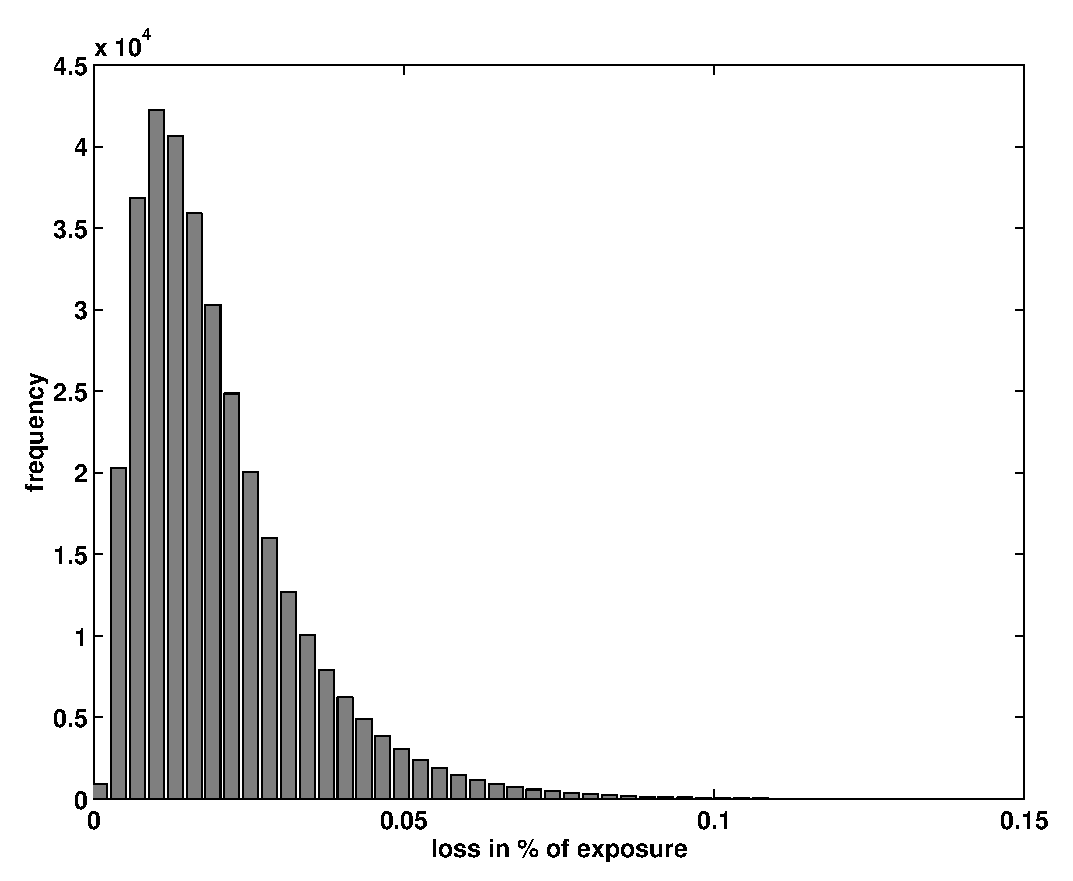
\includegraphics[angle=90,width=7cm,height=7cm,angle=-90]{Chapters/chapter1/figures/Histogram.eps}}
\subfigure[\label{f8b}]{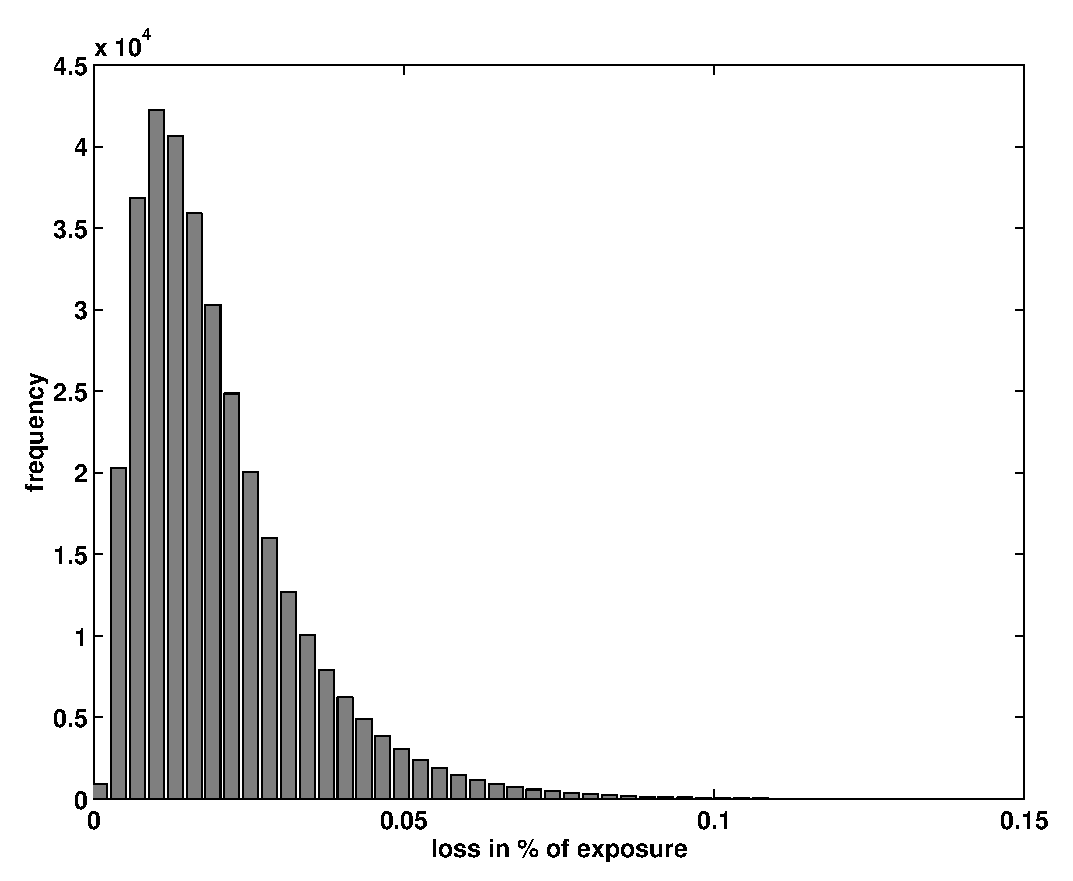
\includegraphics[angle=90,width=7cm,height=7cm,angle=-90]{Chapters/chapter1/figures/Histogram.eps}}
\end{center}
\caption[The bar charts depict the different risk contributions]{The bar charts depict the different risk contributions (top: 99\% quantile, bottom: 99.9\% quantile) of the business areas of a bank. The black bars
are based on a Var/Covar approach, the white ones correspond to shortfall risk.}
\end{figure}

\subsubsection{H3 A component part }
A component part for an electronic item is
manufactured at one of three \cite{mardia1979ma} different factories, and then delivered to
the main assembly line.Of the total number supplied, factory A supplies
50\%, factory B 30\%, and factory C 20\%. Of the components
manufactured at factory A, 1\% are faulty and the corresponding
proportions for factories B and C are 4\% and 2\% respectively. A
component is picked at random from the assembly line. What is the
probability that it is faulty? 


A fundamental notion \cite{yao2002can} is that of a\index{subspace}\index{vector 
space!subspace of} subspace of $F^n$. Let $V$ be a nonempty subset of 
$F^n$. Then $V$ is a {\it subspace} of $F^n$ provided $V$ is closed 
under vector addition and scalar multiplication, that is, 
\begin{enumerate} 
\item[\rm (a)] For all $u$ and $v$ in $V$, $u+v$ is 
also in $V$. 
\item[\rm (b)] For all $u$ in $V$ and $c$ in $F$, $cu$ is 
in $V$. 
\end{enumerate} 
Let $u$ be in the subspace $V$. Because $0u=0$, 
it follows that the zero vector is in $V$. Similarly, $-u$ is in $V$ 
for all $u$ in $V$. A simple example of a subspace of $F^n$ is the set 
of all vectors $(0,a_2,\ldots,a_n)$ with first coordinate equal to 0. 
The zero vector itself is a subspace.

\begin{definition}\label{1def:linearcomb}{\rm
Let $u^{(1)},u^{(2)},\ldots,u^{(m)}$ be vectors in $F^n$, and let 
$c_1,c_2,\ldots,c_m$ be scalars. Then the vector
\[c_1u^{(1)}+c_2u^{(2)}+\cdots+c_mu^{(m)}\]
is called a {\it linear combination} \index{linear combination} of $u^{(1)},u^{(2)},\ldots,u^{(m)}$.
If $V$ is a subspace of $F^n$, then $V$ is closed under vector addition and 
scalar multiplication, and it follows easily by induction that a 
linear combination of vectors in $V$ is also a vector in $V$. Thus 
{\it subspaces 
are closed under linear combinations}; in fact, this can be taken as the 
defining property of subspaces.
The vectors $u^{(1)},u^{(2)},\ldots,u^{(m)}$ {\it span} $V$ \index{spanning set}
(equivalently, form a {\it spanning set} of $V$) provided every vector in 
$V$ 
is a linear combination of $u^{(1)},u^{(2)},\ldots,u^{(m)}$. The zero 
vector can be written as a linear combination of 
$u^{(1)},u^{(2)},\ldots,u^{(m)}$ with all scalars equal to 0; this is a 
{\it trivial linear combination}.\index{linear combination!trivial} The vectors
$u^{(1)},u^{(2)},\ldots,u^{(m)}$ are {\it linearly dependent} provided 
there are scalars $c_1,c_2,\ldots,c_m$, not all of which are zero, such 
that
\[c_1u^{(1)}+c_2u^{(2)}+\cdots+c_mu^{(m)}=0,\]
that is, the zero vector can be written as a {\it nontrivial linear \index{linear combination!nontrivial} 
combination} of $u^{(1)},u^{(2)},\ldots,u^{(m)}$.
For example, the vectors $(1,4), (3,-1)$, and $(3,5)$ in $\Re^2$ are 
linearly 
dependent since
\[3(1,4)+1(3,-2)-2(3,5)=(0,0).\] Vectors are {\it linearly independent} provided  they are not linearly dependent.\index{linearly independent}
The vectors 
$u^{(1)},u^{(2)},\ldots,u^{(m)}$ are a {\it basis} \index{basis} of $V$ provided they are  
linearly independent and span $V$.
By an {\it ordered basis} \index{basis!ordered} we mean a basis in which the vectors of the basis are listed 
in a specified order; to indicate that we have an ordered basis we write
$(u^{(1)},u^{(2)},\ldots,u^{(m)})$. 
A spanning set $S$ of $V$ is a \index{spanning set!minimal} {\it minimal spanning set of $V$} provided that
each set 
of vectors obtained from $S$ by removing a vector is not a spanning set 
for $V$.
A linearly independent set $S$ of vectors of $V$ is a {\it maximal linearly \index{linearly independent!maximal}
independent set of vectors of $V$} provided that for each vector $w$ of 
$V$ that 
is not in $S$, $S\cup\{w\}$ is  linearly dependent (when this happens, 
$w$ must be  a linear combination of the vectors in 
$S$).\hfill{$\Box$}
}\end{definition}

In addition to matrix addition, subtraction, and multiplication, there is 
one additional operation that we define now. It's perhaps the simplest of 
them all. Let $A=[a_{ij}]$ be an $m$ by $n$ matrix and let $c$ be a 
number \cite{hyvarinen2001ica}. Then the matrix $c\cdot A$, or simply $cA$, is the $m$ by $n$ 
matrix obtained by multiplying each entry of $A$ by $c$:
\[c A=[ca_{ij}].\]\index{matrix!scalar multiplication} \index{matrix!scalar multiple of}
The matrix $c A$ is called a {\it scalar multiple} of $A$.

\begin{VT1}

\VH{Think About It...}

Commonly thought of as the first modern computer, ENTAC was built in 1944. It took up more space than an 18-wheeler's
tractor trailer and weighed more than 17 Chevrolet Camaros. It consumed 140,000 watts of electricity while executing
up to 5,000 basic arithmetic operations per second. One of today's popular microprocessors, the 486, is built on a
tiny piece of silicon about the size of a dime.

\VT
With the continual expansion of capabilities, computing power will eventually exceed the capacity for human
comprehension or human control.

\VTA{The Information Revolution}{Business Week}
\end{VT1}


\section{Glossary}
\begin{Glossary}
\item[360 Degree Review] Performance review that includes feedback from superiors, peers, subordinates, and clients.
\item[Abnormal Variation] Changes in process performance that cannot be accounted for by typical day-to-day variation. Also referred to as
non-random variation.
\item[Acceptable Quality Level (AQL)] The minimum number of parts that must comply with quality standards, usually stated as a percentage.
\item[Activity] The tasks performed to change inputs into outputs.
\item[Adaptable] An adaptable process is designed to maintain effectiveness and efficiency as requirements change. The process is
deemed adaptable when there is agreement among suppliers, owners, and customers that the process will meet
requirements throughout the strategic period.
\end{Glossary}




%\include{chapters/chapter2/ch2}

\bibliographystyle{plain}
\bibliography{bibtex_example}

\printindex

\end{document}
